\documentclass[a0paper]{baposter}

\usepackage{lipsum}
\usepackage{graphicx}
\graphicspath{{images/}{../images/}}

\begin{document}

%:Background image
\background{
      \begin{tikzpicture}[remember picture,overlay]%
      \draw (current page.north west)+(-2em,2em) node[anchor=north west]
      {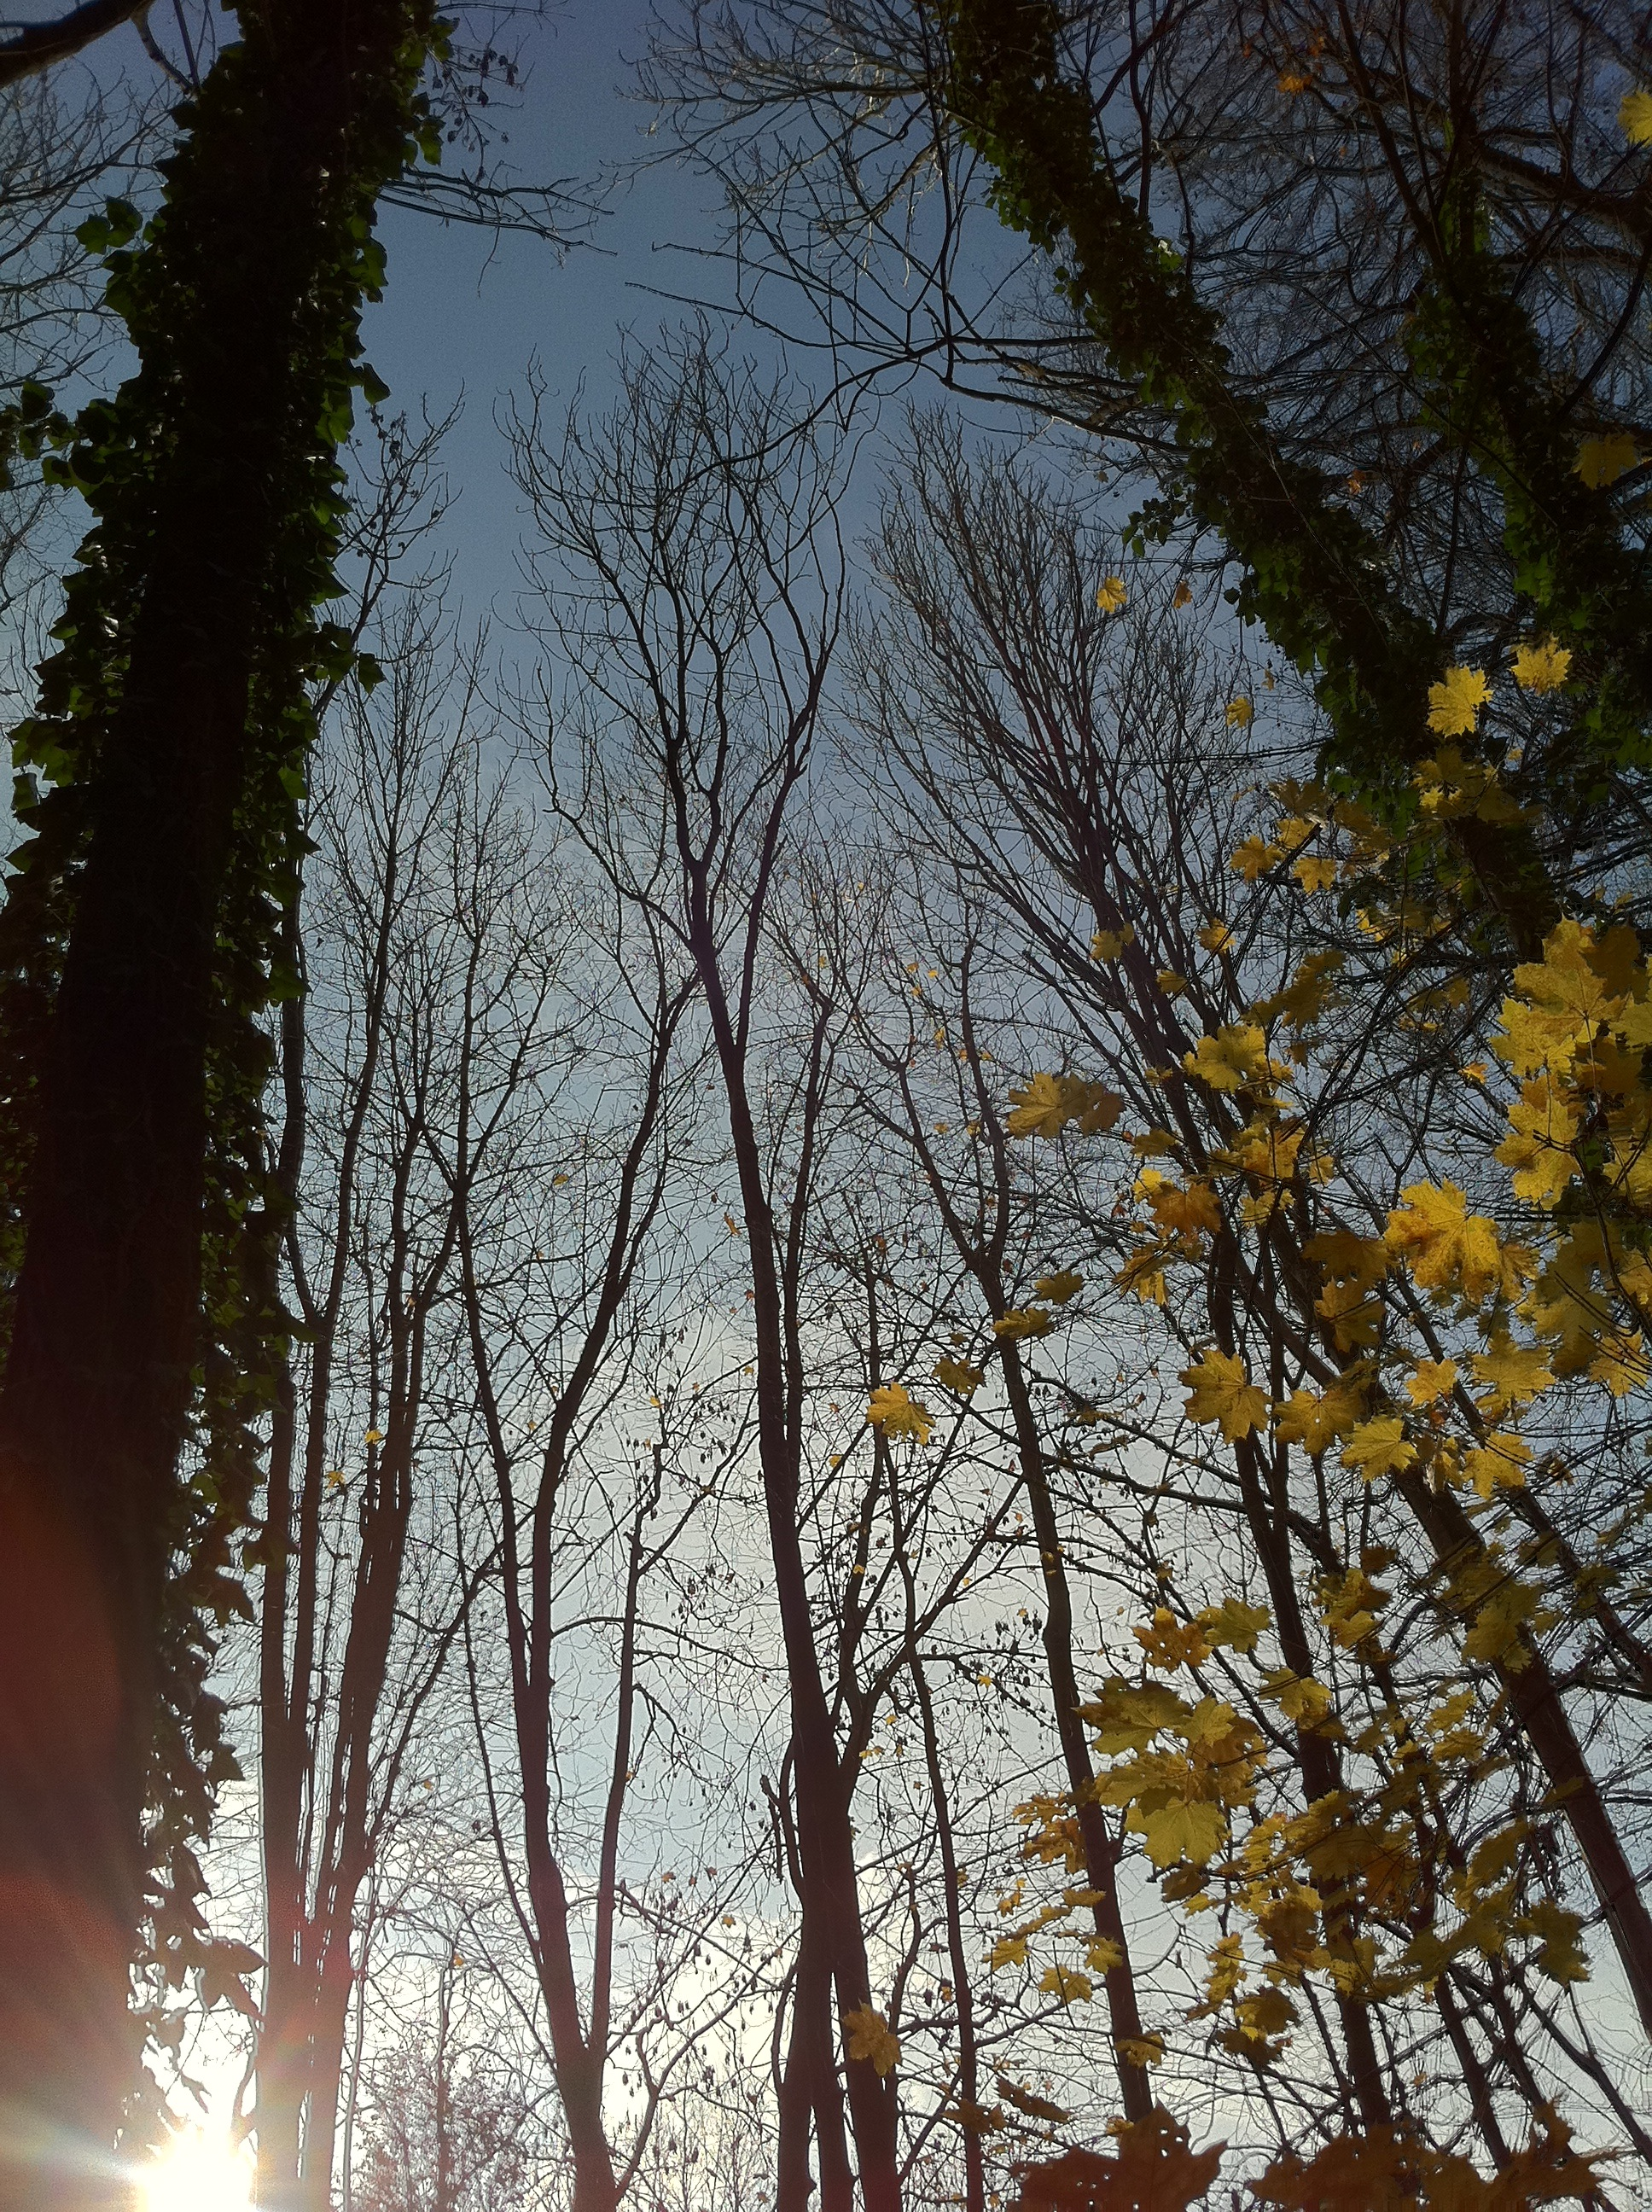
\includegraphics[height=1.1\textheight]{trees.jpg}};
      \end{tikzpicture}%
      }
\begin{poster}{
headershade=plain,
headerColorOne=green,
headerFontColor=white,
boxshade=plain,
headerfont=\Large\bfseries,
background=user,
% Adjust transparency of text boxes
boxopacity=.75,
textborder=none,
boxColorOne=white
}
	{}
	{\color{white}Transparent Box Example}
	{\color{white}Mathias Loesch}
	{}
\headerbox{Text Box}{name=b1,column=0,row=0, span=1}
{\lipsum[1]}
%
\headerbox{Text Box}{name=b2,below=auto}
{\lipsum[2]}
%
\headerbox{Text Box}{name=b3, span=2, column=1}
{\lipsum[3]}


\end{poster}
\end{document}